\documentclass[a4paper,12pt]{article}

\usepackage[utf8]{inputenc}
\usepackage[T1]{fontenc}
\usepackage{amsmath, amssymb}
\usepackage{graphicx}
\usepackage{hyperref}
\usepackage{geometry}
\geometry{a4paper, margin=1in}
\usepackage{subcaption}
\usepackage{csvsimple}
\usepackage{float}

\title{Gaussian Mixture Model Report}
\author{Eduardo}
\date{\today}

\begin{document}

\maketitle

\section{Introduction}
This report describes the application of Gaussian Mixture Models (GMMs) and K-Means for classifying spiral-shaped data. The proposed BayesGMM classifier combines class-specific GMMs for prediction, using cross-validation to optimize hyperparameters. Results demonstrate high accuracy in class separation.

\section{Methodology}
\subsection{Data Generation}
Synthetic spiral data were generated with added Gaussian noise. Each class was rotated 180 degrees to create nonlinear separation.

\subsection{Clustering and Modeling}
\begin{itemize}
  \item \textbf{K-Means}: Applied separately to each class to identify 8 clusters.
  \item \textbf{GMM}: Fitted to each class with 8 components, capturing covariance structures.
  \item \textbf{BayesGMM}: Classifier combining class-specific GMM likelihoods, weighted by priors.
\end{itemize}

\subsection{Evaluation}
Grid search (\textit{GridSearchCV}) determined the optimal number of components (8). Accuracy was validated via 10-fold cross-validation.

\section{Results}
\subsection{Cluster Visualization}
\begin{figure}[H]
  \centering
  \begin{subfigure}{0.45\textwidth}
    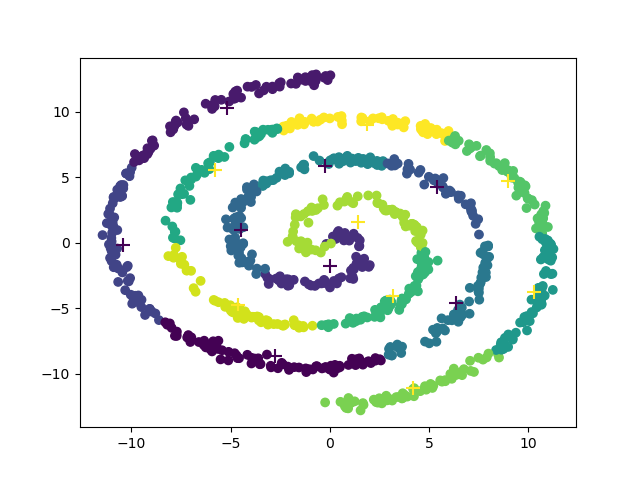
\includegraphics[width=\textwidth]{kmeans.png}
    \caption{Clusters identified by K-Means}
    \label{fig:kmeans}
  \end{subfigure}
  \hfill
  \begin{subfigure}{0.45\textwidth}
    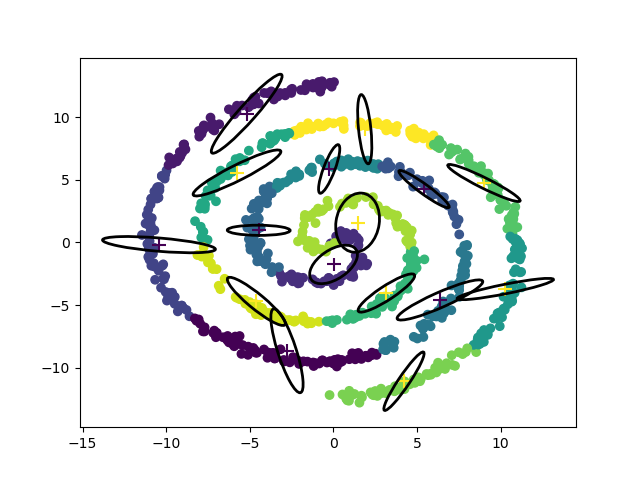
\includegraphics[width=\textwidth]{kmeans_ellipses.png}
    \caption{Covariance ellipses (K-Means)}
    \label{fig:kmeans_ellipses}
  \end{subfigure}
  \vspace{5mm}
  \begin{subfigure}{0.45\textwidth}
    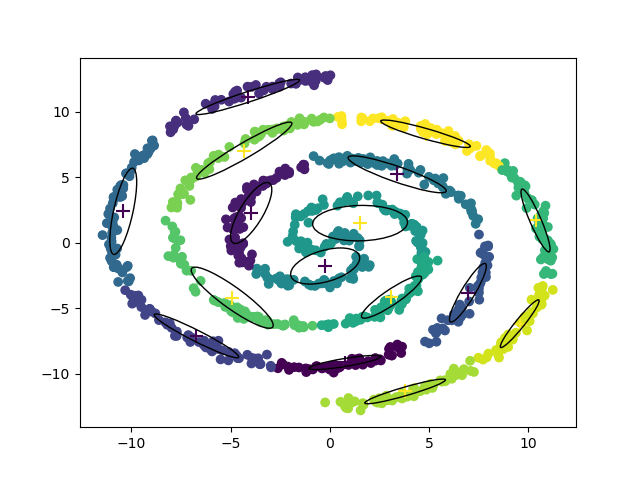
\includegraphics[width=\textwidth]{gmm_ellipses.png}
    \caption{GMM components with ellipses}
    \label{fig:gmm_ellipses}
  \end{subfigure}
  \hfill
  \begin{subfigure}{0.45\textwidth}
    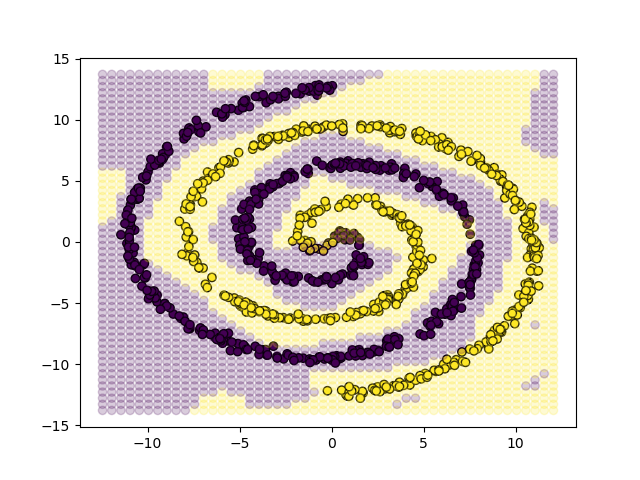
\includegraphics[width=\textwidth]{gmm_dec_bound.png}
    \caption{BayesGMM decision boundary}
    \label{fig:dec_bound}
  \end{subfigure}
  \caption{Model visualizations}
\end{figure}

\subsection{Performance}
\begin{table}[H]
  \centering
  \caption{Accuracy per Cross-Validation Fold}
  \label{tab:scores}
  \csvautotabular{scores.csv}
\end{table}

\section{Conclusion}
The BayesGMM model achieved a mean accuracy of 99\%, demonstrating effectiveness in classifying nonlinear data. The multi-component per-class structure successfully captured spiral complexity. Hyperparameter optimization validated the choice of 8 components per class.

\end{document}
